% !TeX program  = xelatex
% !TeX encoding = UTF-8
% !TeX root     = 1_nft_tokenomics.tex
\documentclass{mirea-article}

% !TeX program  = xelatex
% !TeX encoding = UTF-8
% !TeX root     = final-qualifying-work.tex

\usepackage{hyperref}
\urlstyle{same}

\hypersetup{
    pdftoolbar=true,        % show Acrobat’s toolbar?
    pdfmenubar=true,        % show Acrobat’s menu?
    pdffitwindow=false,     % window fit to page when opened
    pdfstartview={FitH},    % fits the width of the page to the window
    pdftitle={ВКР на тему "Разработка системы токенизации дипломов на основе блокчейн-технологий для цифровой верификации и децентрализованного хранения образовательных достижений"},
    pdfauthor={М. Д. Панфилов},
    pdfsubject={Qualification Collectibles},
    pdfcreator={mxp@apteryx},
    pdfproducer={XeLaTex in VSCode},
    pdfkeywords={final qualifying work} {nft diplomas} {qualification collectibles} {educational nft}, 
    pdfnewwindow=true
}

\usepackage{comment}

\usepackage{etoolbox}

\usepackage{graphicx}

\usepackage{listings}
\usepackage{xcolor}
\lstset{basicstyle=\footnotesize, breaklines=true, numbers=left, captionpos=t, showstringspaces=false, commentstyle=\color{teal}, stringstyle=\color{red}, keywordstyle=\color{violet}}  % Настройки для всех листингов

% Введение и заключение
\newcommand{\supersection}[1]{
	\section*{#1}
	\phantomsection
	\addcontentsline{toc}{section}{#1}
}

\usepackage{caption}
\captionsetup[lstlisting]{justification=raggedright, singlelinecheck=false}

\usepackage{pdfpages}

\usepackage{microtype}

\tolerance=5000
\hbadness=9999
\emergencystretch=10pt
\hyphenpenalty=5000
\exhyphenpenalty=100

\usepackage{multirow}

\usepackage{array}
\usepackage{setspace}
\newcolumntype{x}[1]{>{\setstretch{0.8}\small\centering\arraybackslash\hspace{0pt}}m{#1}}
\newcolumntype{y}[1]{>{\centering\arraybackslash\hspace{0pt}}m{#1}}
\usepackage{longtable}

\usepackage{float}

\usepackage{listings}
\usepackage{xcolor}
\lstset{basicstyle=\footnotesize, breaklines=true, numbers=left, captionpos=t, showstringspaces=false, commentstyle=\color{teal}, stringstyle=\color{red}, keywordstyle=\color{violet}} % Настройки для всех листингов
\usepackage{caption}
\captionsetup[lstlisting]{justification=raggedright, singlelinecheck=false}

%\usepackage{color,xesearch}
%\SearchList{make-red}{\textcolor{red}{#1}}{эффективность,качество}
\usepackage{multicol}
\usepackage{ragged2e}

\newenvironment{Figure}
{\par\medskip\noindent\minipage{\linewidth}}
{\endminipage\par\medskip}

\begin{document}

\textbf{УДК 378, 004.62}

\artauthor{Люцько Сергей Алексеевич}{Студент специальности <<Информационные системы и технологии>> ИКБ РТУ МИРЭА}{ouhguy@gmail.com}

\artauthor{Панфилов Максим Дмитриевич}{Студент специальности <<Информационные системы и технологии>> ИКБ РТУ МИРЭА}{panfilov.m.d@edu.mirea.ru}

\artauthor{Котилевец Игорь Денисович}{Научный руководитель, старший преподаватель кафедры ИКБ РТУ МИРЭА}{ikotilevets@gmail.com}


\supersection{Применение токеномики и nft для верификации дипломов высшего учебного заведения и выявления приоритетов развития студентов.}

Аннотация. {\itshape Современное общество столкнулось c незаконным бизнесом, связанным с торговлей поддельными дипломами различных образовательных учреждений. Эта деятельность предоставляет иллюзорную возможность обойти требования образовательного процесса, приобретя фальшивый диплом, и трудоустроиться без должного уровня квалификации. Такое состояние дел ведёт к проникновению неквалифицированных специалистов в различные области деятельности. Последствия такой ситуации могут быть различными, начиная с отсутствия негативного воздействия вплоть до крайне серьёзных проблем, например, некомпетентность медицинских специалистов, от решений которых зависят жизни людей.
\par Существующая система подтверждения подлинности дипломов является недостаточной, а законодательные нормы позволяют лицам, получившим работу с использованием поддельных дипломов, продолжать свою профессиональную деятельность в определённых обстоятельствах.
\par Технологии блокчейн предлагают возможность фундаментального изменения текущей ситуации, обеспечивая прозрачность и неизменность данных об образовательных достижениях каждого индивидуума, что может служить эффективной мерой против распространения поддельных дипломов.}

Ключевые слова: \textit{подделка дипломов, блокчейн, технология распределённого реестра, невзаимозаменяемые токены.}

\supersection{The use of tokenomics and NFT to verify diplomas of higher education institutions and identify priorities for student development.}

Annotation. {\itshape Contemporary society is grappling with the illicit business of trafficking counterfeit diplomas from various educational institutions. This activity offers the illusory chance to circumvent the requirements of the educational process by acquiring a fake diploma, enabling individuals to gain employment without the requisite level of qualification. Such a state of affairs leads to the infiltration of unqualified professionals across various sectors. The repercussions of this scenario can vary widely, ranging from negligible impact to extremely serious issues, such as the incompetence of medical professionals whose decisions can be life-critical.
\par The current system for verifying the authenticity of diplomas is inadequate, and legislative norms allow individuals who have secured employment using fake diplomas to continue their professional activities under certain circumstances.
\par Blockchain technology presents the potential for a fundamental change in this situation by ensuring transparency and immutability of data regarding each individual's educational achievements, which could serve as an effective measure against the proliferation of counterfeit diplomas.}

Keywords: \textit{diploma forgery, blockchain, distributed ledger technology, non-interchangeable tokens.}

\subsection*{Введение}
\label{sec:introduction}

Современное общество характеризуется акцентом на образование как на ключевой инструмент для социальной мобильности и профессионального успеха. Однако, несмотря на это, феномен подделки академических документов представляет собой значительную проблему. Индивиды, прибегающие к приобретению поддельных дипломов, преодолевают образовательные барьеры, апеллируя к недостоверной документации для подтверждения их профессиональной квалификации. Данное нарушение, называемое академическим мошенничеством, представляет серьезное преступление и влечет за собой негативные последствия.

Статистика по таким делам не публикуется, однако некоторые случаи трудоустройства по поддельным дипломам всё же были преданы огласке. ~\cite{bib:korochka-ne-glavnoe, bib:nursing-diploma-scheme}

Самая простая процедура проверки диплома на подлинность в России – обращение к Федеральному реестру сведений о документах об образовании и (или) о квалификации, документах об обучении (ФИС ФРДО) через сайт Рособрнадзора. Для этого потребуются по меньшей мере такие данные, как ФИО получателя диплома, указание уровня образования, название высшего учебного заведения, регистрационный номер и гос. серия диплома, а также дата выдачи. Этот способ проверки имеет определённый ряд ограничений: несмотря на загрузку информации в базу, нельзя проверить дипломы, полученные в вузах научных организаций. Информация о структурных подразделениях, находящихся под управлением Федеральной службы безопасности Российской Федерации или Службы внешней разведки, недоступна для проверки, поскольку является объектом государственной секретности. ~\cite{bib:proverka-diplomov}

Альтернативные методы верификации включают в себя процедуру направления письменных заявлений к различным учреждениям и требуют значительного времени на ожидание соответствующего ответа.

Высшие учебные заведения обычно используют бумажные бланки для хранения и выдачи дипломов, что увеличивает стоимость выпуска, хранения, передачи и аудита этих документов. Этот метод также не гарантирует их сохранность и требует использования сертификационных центров для проверки печатей и подписей, что влечёт за собой потенциальные уязвимости.

\subsection*{Основная часть}

Выделяют три области применения технологии распределённых реестров (блокчейн).

\textit{Блокчейн 1.0} – это валюта. Криптовалюты применяются в различных приложениях, имеющих отношение к деньгам, например системы переводов и цифровых платежей.

\textit{Блокчейн 2.0} – это контракты. Целые классы экономических, рыночных и финансовых приложений, в основе которых лежит блокчейн, работают с различными типами финансовых инструментов – с акциями, облигациями, фьючерсами, закладными, правовыми титулами, умными активами и умными контрактами.

\textit{Блокчейн 3.0} – это приложения, область применения которых выходит за рамки денежных расчетов, финансов и рынков. Они распространяются на сферы государственного управления, здравоохранения, науки, образования, культуры и искусства.~\cite{bib:swan-chain}

Именно третья область может оказаться полезной в решении рассматриваемой проблемы, и в настоящее время технологии распределённых реестров (блокчейн) уже активно внедряются в сферу образования.~\cite{bib:blokchejn-v-obrazovanii, bib:blokcheyn-v-uchebnom-protsesse}

Массачусетский технологический университет (MIT) в сотрудничестве с компанией по разработке программного обеспечения <<Learning Machine>> в рамках пилотного проекта выдал 111 цифровых дипломов. Эти дипломы были выпущены на основе сети Bitcoin через приложение Blockcerts Wallet, обеспечивающее обладателю такого виртуального документа его надёжное хранение и защиту от несанкционированного доступа~\cite{bib:mit-diplomas}. Информация о таком дипломе не хранится в блокчейне, система использует транзакции с временными метками, указывающими на то, что именно MIT создал цифровую запись для сертификата. Предоставляется сайт для проверки сертификатов: https://credentials.mit.edu.

Следом же за MIT – Министерство образования и занятости Мальты и Австралийский университет в Мельбурне приступили к тестированию Blockcerts для отслеживания академических сертификатов.

Точных аналогов данному методу не было обнаружено, однако существуют косвенные аналогии на уровне концептуальных идей, указанные в источниках.~\cite{bib:nfts-replace-diplomas, bib:nfts-and-higher-education}

В ответ на вышеуказанную проблему предлагается инновационное решение, основанное на использовании технологии невзаимозаменяемых токенов (Non-Fungible Tokens, NFT). Согласно предложенной концепции, каждый NFT будет генерироваться по унифицированному алгоритму, однако параметры каждого токена будут разниться. Эта особенность позволяет обеспечить уникальность каждого образовательного аккредитива, существенно усложняя его подделку и предоставляя надежное средство верификации академических достижений.

Так, формирующее и выпускающее подразделения, вид образовательной программы, форма обучения, специальность, номер группы, ФИО или любые другие идентификационные данные студента будут влиять на визуальную составляющую генерируемого изображения, а специфическая строка данных, именуемая солью, будет гарантировать его уникальность. Бóльшую функциональность такого токена можно обеспечить, реализовав его кастомизацию также относительно общественно полезной деятельности, в которую студент был вовлечён на протяжении учебного процесса. Так, токен сможет отражать в качестве полезной для работодателя информации приоритеты развития студента.

Храниться эти изображения будут с использованием IPFS (InterPlanetary File System) – протокола и одноранговой сети для хранения и обмена данными в распределенной файловой системе. IPFS использует контент-адресацию для уникальной идентификации каждого файла в глобальном пространстве имен, соединяющем все вычислительные устройства. Каждое хранимое изображение будет сопровождаться метаданными, представленными в виде хэша от идентификационных данных студента, что откроет возможность проводить обратную верификацию таких NFT-дипломов.

Для обеспечения качества выдачи дипломов целесообразно разработать специализированный блокчейн для высших учебных заведений или использовать единую государственную сеть, например, российскую сертифицированную высокопроизводительную блокчейн-платформу для создания бизнес-приложений MasterChain~\cite{bib:masterchain}. Такой подход имеет цель разгрузить публичные сети, как Ethereum или Bitcoin. Однако в контексте собственной сети возникает проблема: убедить большинство университетов, школ или образовательных курсов присоединиться к частному блокчейну становится непростой задачей. А сеть MasterChain ещё не запущена. Для решения этого вопроса можно использовать сети вроде TON или Polygon.

Чтобы создать необходимый токен, студенту будет предоставлен специальный код доступа, который позволит им самостоятельно <<минтить>> (принимать участие в первичном распределении токенов) свой токен в официальной коллекции (наборе неограниченного количества невзаимозаменяемых токенов, объединённых общей темой) учебного заведения. Поскольку специфика блокчейн сетей подразумевает оплату данного процесса, со стороны студента потребуется оплата пошлины. На вуз же возляжет обязанность ежегодно выпускать коллекции для таких дипломов, оплачивая их выпуск.

\begin{table}[htb]
    \caption{Сравнение стоимости создания коллекции и выпуска токена (цены актуальны на 29.05.2023)}
    \centering
    \setlength{\tabcolsep}{10pt} % Увеличение отступа между столбцами
    \renewcommand{\arraystretch}{1.5} % Увеличение высоты строк

    \begin{tabular}{|c|c|c|c|c|c|}
        \hline
        \multirow{2}{*}{\textbf{Сеть}} & \multirow{2}{*}{\textbf{Токен}} & \multicolumn{2}{c|}{\textbf{Создание коллекции}} & \multicolumn{2}{c|}{\textbf{Выпуск токена}} \\ \cline{3-6} 
         &  & \small{\textbf{Криптовалюта}} & \small{\textbf{Рубли}} & \small{\textbf{Криптовалюта}} & \small{\textbf{Рубли}} \\ \hline
        \textbf{Ethereum} & ETH & 0.04-0.06 & 6100-9100 & 0,02+ & 2400+ \\ \hline
        \textbf{Polygon} & MATIC & 0.2-0.5 & 15-50 & 0.05-0.15 & 4-11 \\ \hline
        \textbf{TON} & TON & 0.05-0.2 & 7.5-30 & 0.14-0.29 & 7.59-30.09 \\ \hline
    \end{tabular}
\end{table}

\begin{figure}[htb]
    \centering
    \setlength\fboxsep{2pt} % Отступ между изображением и рамкой
    \setlength\fboxrule{0.5pt} % Толщина рамки
    \begin{minipage}{.5\textwidth}
        \centering
        \fbox{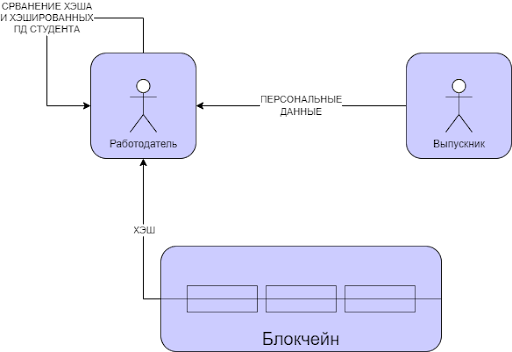
\includegraphics[height=5cm, keepaspectratio]{diploma_verify}}
        \captionof{figure}{Верификация диплома}
        \label{fig:diploma-verify}
    \end{minipage}%
    \begin{minipage}{.5\textwidth}
        \centering
        \fbox{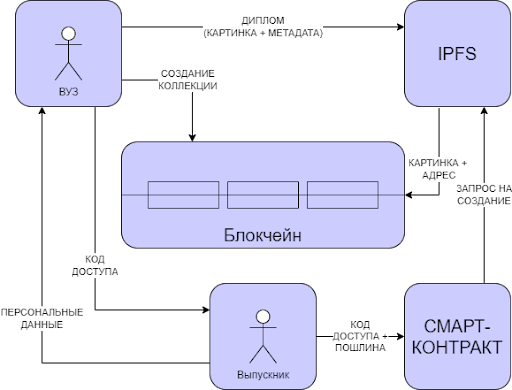
\includegraphics[height=5cm, keepaspectratio]{token_creation}}
        \captionof{figure}{Создание токена диплома}
        \label{fig:token-creation}
    \end{minipage}
\end{figure}


\subsection*{Вывод}

Таким образом, были выявлены предпосылки к использованию технологий распределённых реестров в процессе верификации документов о высшем образовании, а также предложена идея потенциального решения проблемы их фальсификации.

\begin{thebibliography}{99\kern\bibindent}
	\bibitem{bib:korochka-ne-glavnoe} Суд разъяснил, в каком случае уволят за поддельный диплом // rg.ru URL: \url{https://rg.ru/2022/12/12/korochka-ne-glavnoe.html} (дата обращения: 22.05.2023).

	\bibitem{bib:nursing-diploma-scheme} Feds announce massive takedown of fraudulent nursing diploma scheme // ABC News URL: \url{https://abcnews.go.com/US/feds-announce-massive-takedown-fraudulent-nursing-diploma-scheme/story?id=96619487} (дата обращения: 22.05.2023).

	\bibitem{bib:proverka-diplomov} Проверить диплом на подлинность в госреестре ФИС ФРДО // Прикамский институт безопасности дистанционное обучение URL: \url{https://pib24.ru/articles/novosti/proverka-diplomov} (дата обращения: 22.05.2023).

	\bibitem{bib:swan-chain} Свон М. "Блокчейн: Схема новой экономики." – М.: «Олимп–Бизнес» (2017): 240.

	\bibitem{bib:blokchejn-v-obrazovanii} Как используются блокчейн-разработки в образовании // Be(In)Crypto URL: \url{https://ru.beincrypto.com/blokchejn-v-obrazovanii} (дата обращения: 22.05.2023).

	\bibitem{bib:blokcheyn-v-uchebnom-protsesse} Новосёлова Д. В., Тагирова Н. М. Применение технологии блокчейн в учебном процессе // Теория и практика социогуманитарных наук. 2020. №2 (10): 48-50. % https://cyberleninka.ru/article/n/primenenie-tehnologii-blokcheyn-v-uchebnom-protsesse
	
	\bibitem{bib:mit-diplomas} MIT to Issue Diplomas Using Bitcoin Blockchain // Bitcoin.com URL: \url{https://news.bitcoin.com/mit-issue-diplomas-using-bitcoin-blockchain} (дата обращения: 22.05.2023).

	\bibitem{bib:nfts-replace-diplomas} Education NFTs Will Replace Diplomas and Resumes // LinkedIn URL: \url{https://www.linkedin.com/pulse/education-nfts-replace-diplomas-resumes-beau-brannan} (дата обращения: 22.05.2023).

	\bibitem{bib:nfts-and-higher-education} NFTs and Higher Education // NonFungible URL: \url{https://nonfungible.com/news/opinions/nfts-and-higher-education-part-1} (дата обращения: 22.05.2023).

	\bibitem{bib:masterchain} Блокчейе-платформа мастерчейн // MasterChain URL: \url{https://www.masterchain.ru/products/masterchain} (дата обращения: 22.05.2023).
\end{thebibliography}

\end{document}